
\section{Comparison with observations}
\label{sec:comp-with-observ}


Placing various classes of objects on the \(R_{90}\)--\(R_c\) plane:
\begin{itemize}
\item LL arcs
\item runaway O stars
\item AGB stars
\end{itemize}

\subsection{Mid-infrared arcs around early-type stars}
\label{sec:mid-infrared-arcs}

\begin{figure}
  (a)\\
  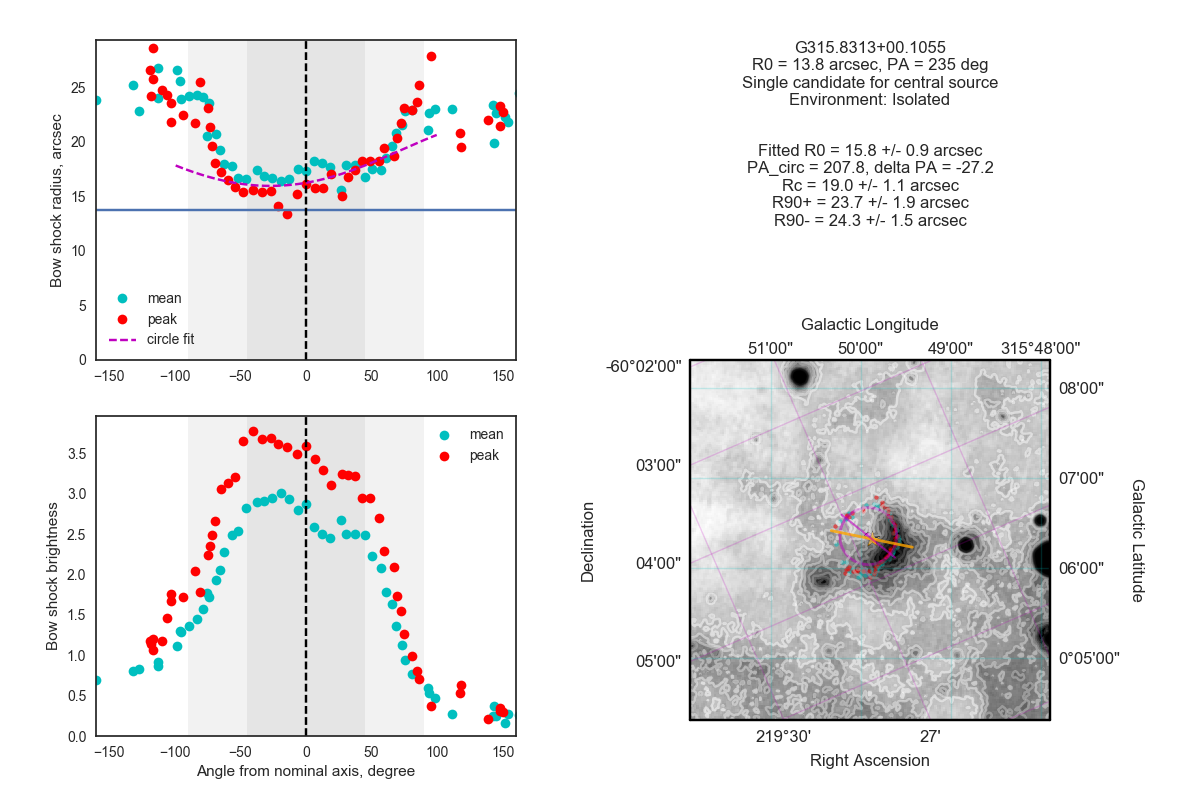
\includegraphics[width=\linewidth]{figs/0510-3-star}
  (b)\\
  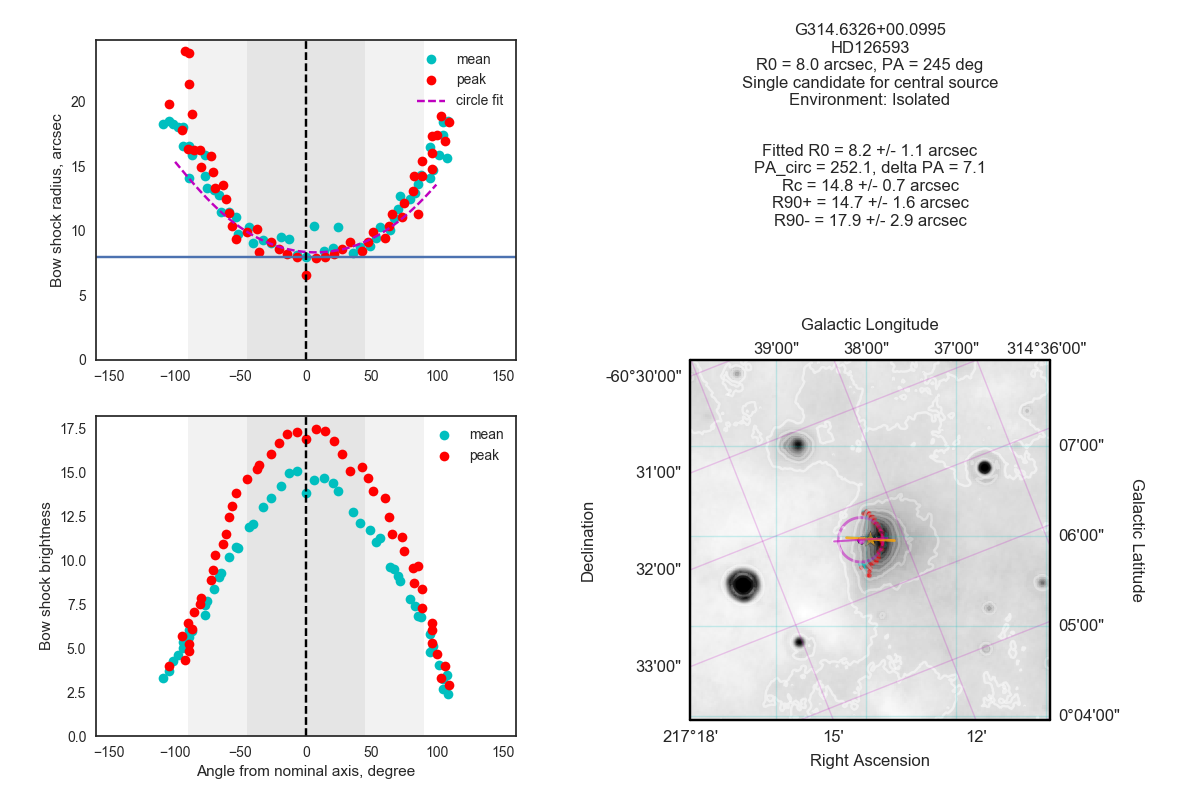
\includegraphics[width=\linewidth]{figs/0506-4-star}
  (c)\\
  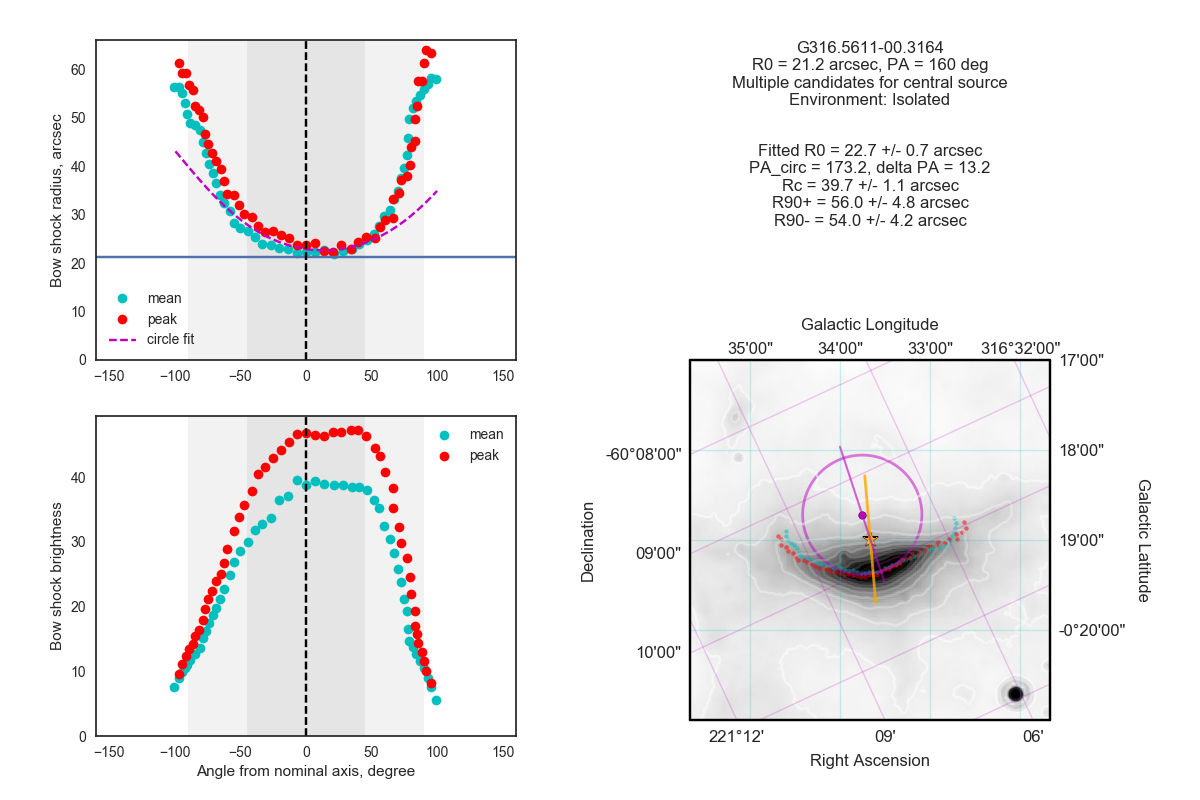
\includegraphics[width=\linewidth]{figs/0517-5-star}
  \caption[]{Examples of fits to the bow shock shapes of MIPSGAL sources.}
  \label{fig:mipsgal-examples}
\end{figure}


\begin{figure}
  \centering
  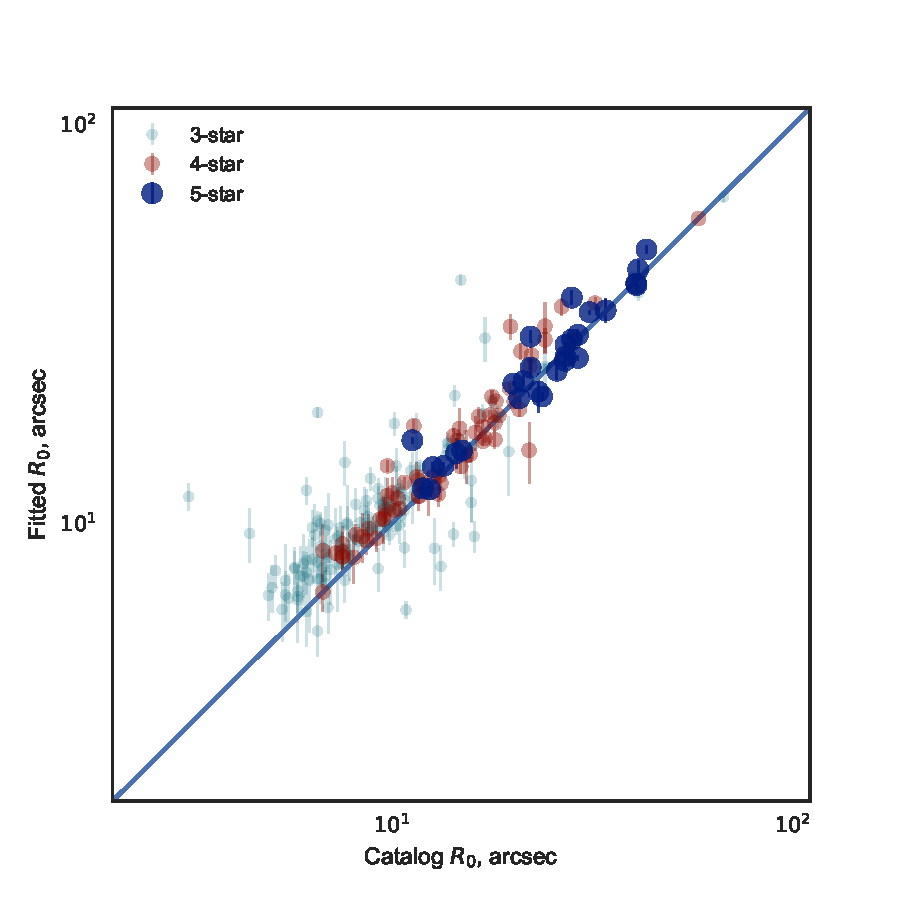
\includegraphics[width=\linewidth]{figs/mipsgal-r0-r0}
  \caption[]{Comparison of the bow shock sizes determined from our fits
    with those given by Kobulnicky for the MIPSGAL sources.}
  \label{fig:mipsgal-sizes}
\end{figure}


\begin{figure*}
  \centering
  \begin{tabular}{ll}
    (a) & (b) \\
    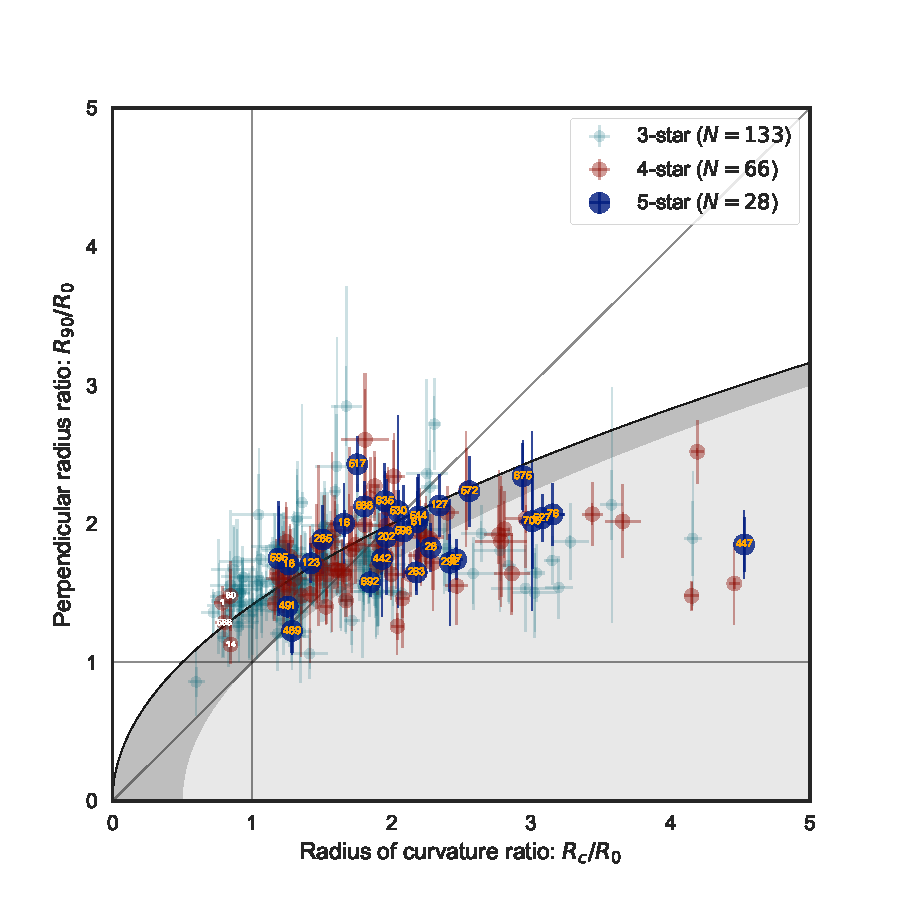
\includegraphics[width=0.45\textwidth]{figs/mipsgal-Rc-R90-zoom} &
    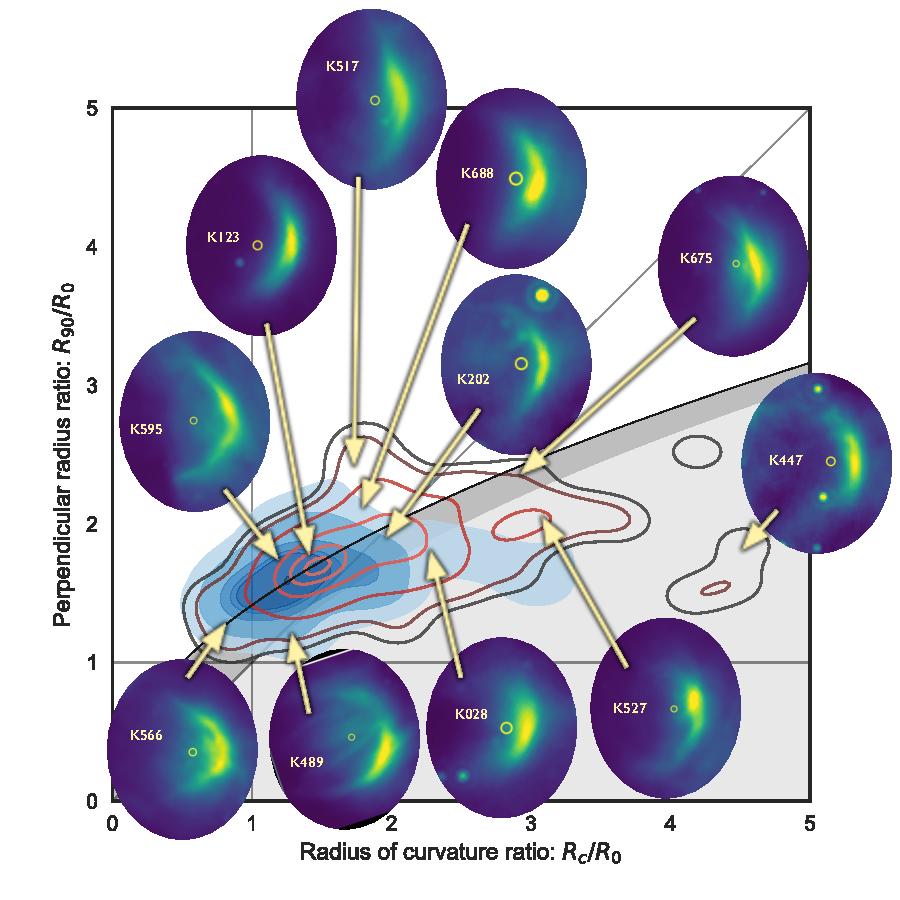
\includegraphics[width=0.45\textwidth]{figs/mipsgal-Rc-R90-thumbnails} 
  \end{tabular}
  \caption[]{MIPSGAL sources on the bow shock shape diagnostic
    diagram.  (a) Individual sources.  (b) Kernel density estimate of
    the distribution.}
  \label{fig:mipsgal-shapes}
\end{figure*}


\begin{figure*}
  \centering
  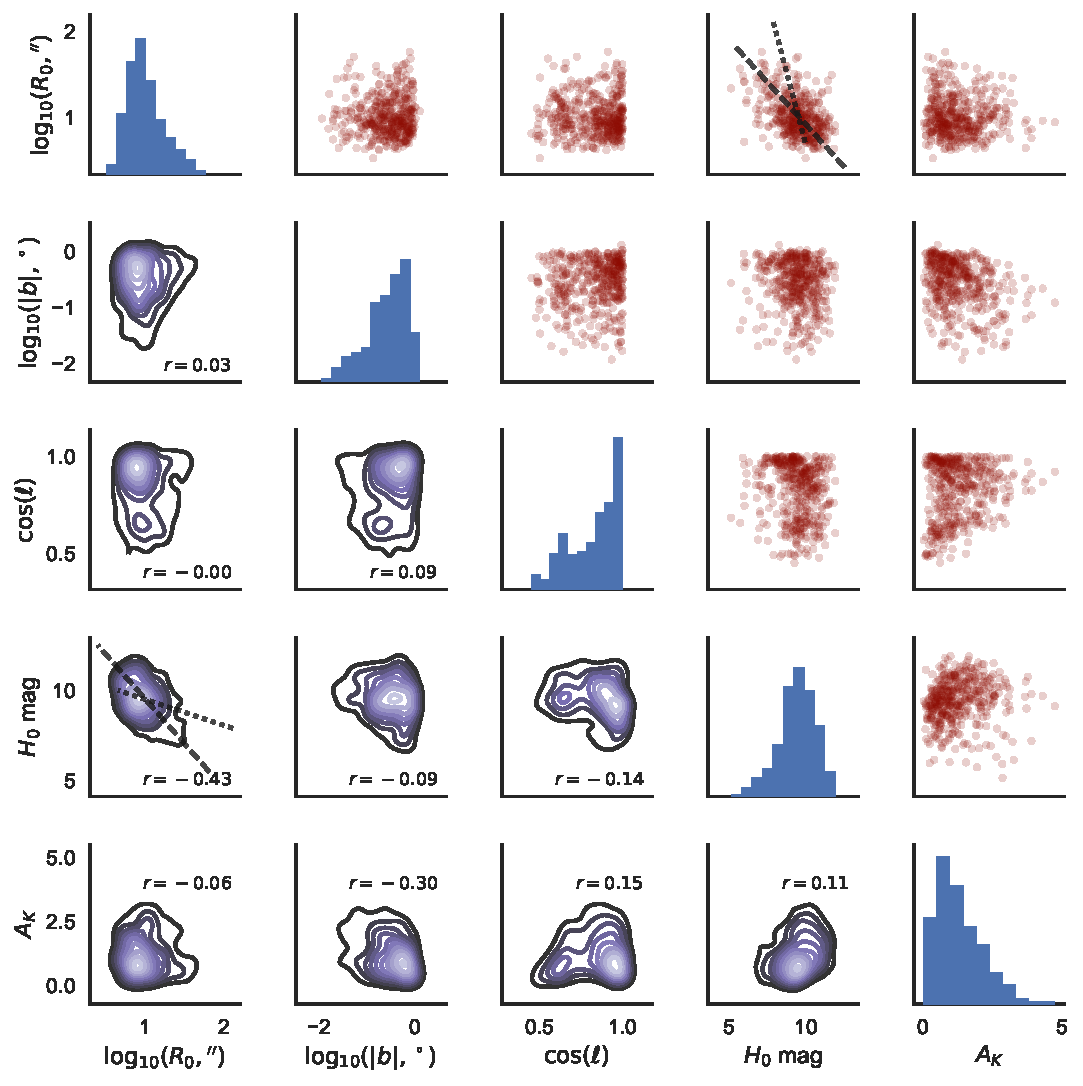
\includegraphics[width=\textwidth]{figs/mipsgal-pairplot}
  \caption[]{Correlations between non-shape parameters of MIPSGAL sources.}
  \label{fig:mipsgal-pairplot}
\end{figure*}

\begin{figure*}
  \centering
  \begin{tabular}{ll}
    (a) & (b) \\
    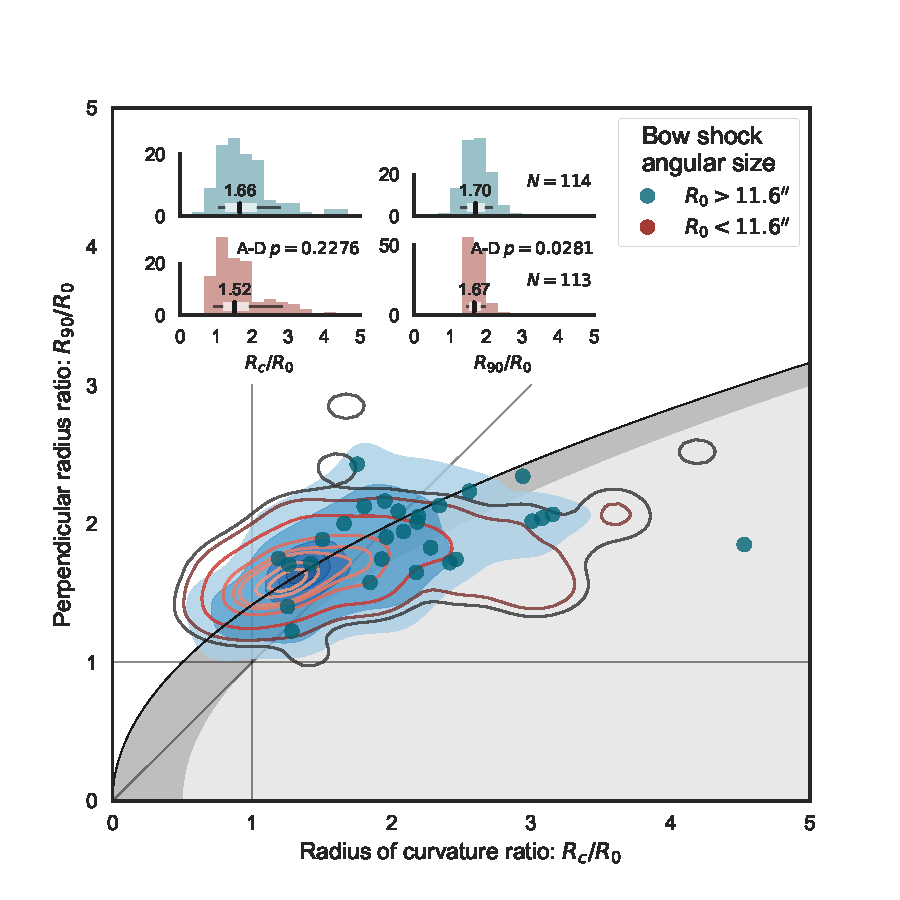
\includegraphics[width=0.45\textwidth]{figs/mipsgal-Rc-R90-R0} &
    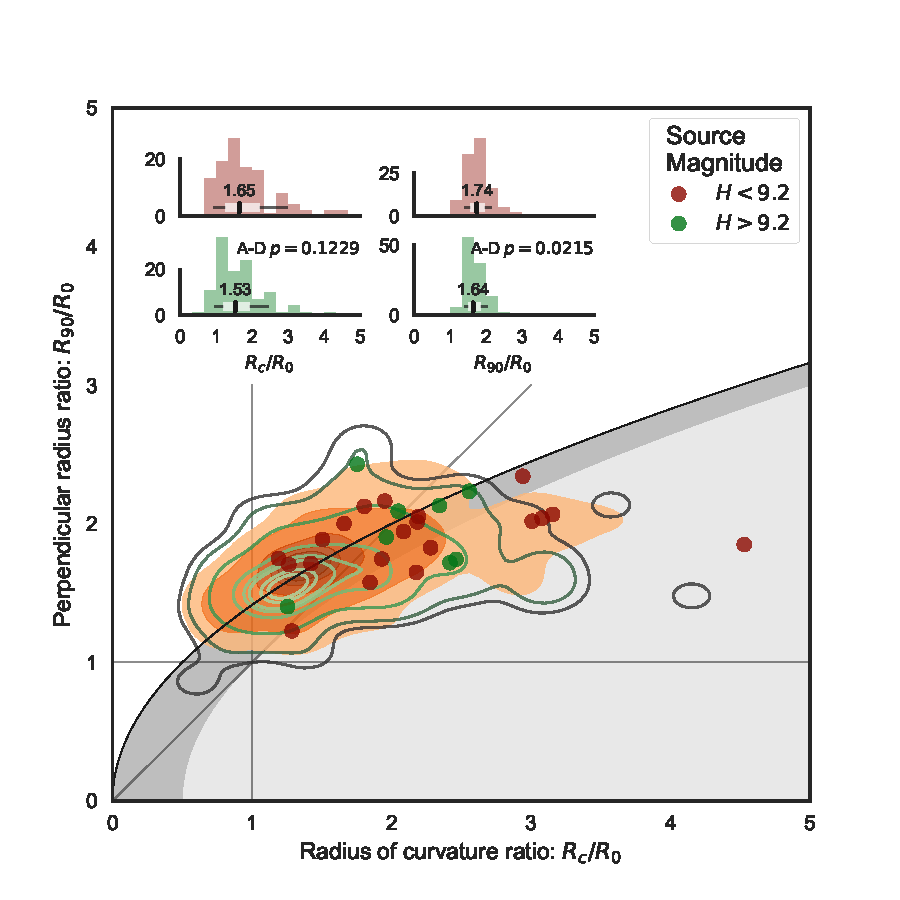
\includegraphics[width=0.45\textwidth]{figs/mipsgal-Rc-R90-Mag} 
  \end{tabular}
  \caption[]{Significant correlation of bow shock shape with (a) bow
    shock angular size, and (b) extinction-corrected magnitude of
    stellar source.}
  \label{fig:mipsgal-correlated}
\end{figure*}

\begin{figure*}
  \centering
  \begin{tabular}{ll}
    (a) & (b) \\
    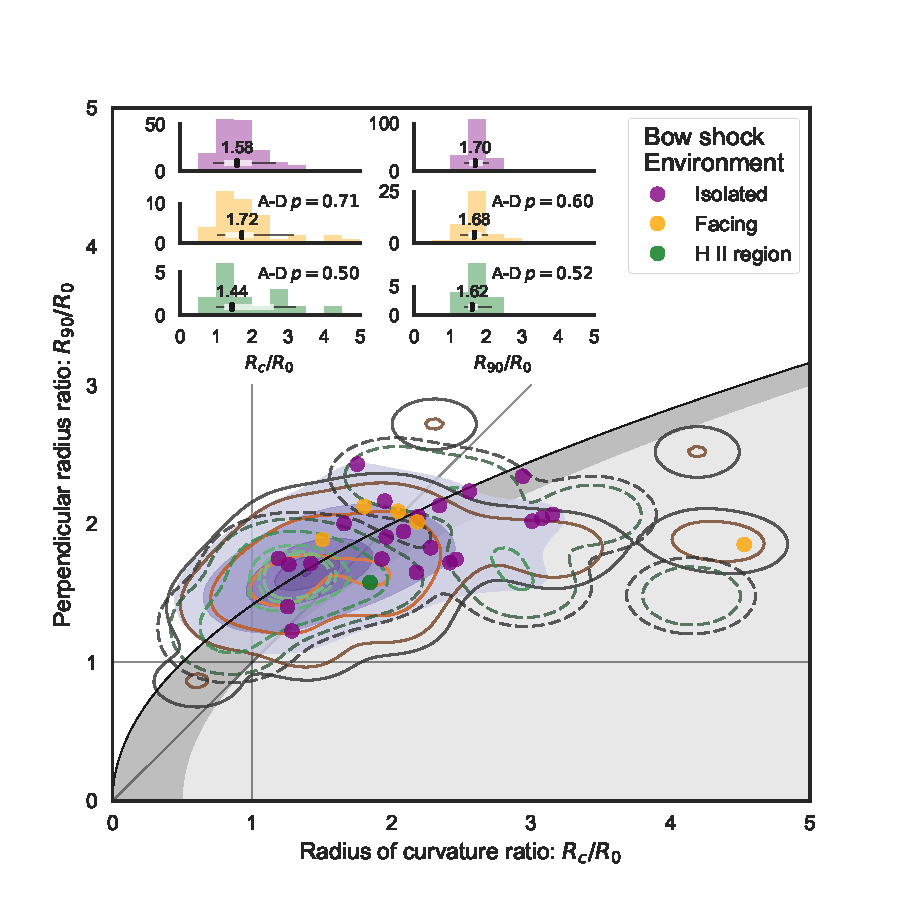
\includegraphics[width=0.45\textwidth]{figs/mipsgal-Rc-R90-environment} &
    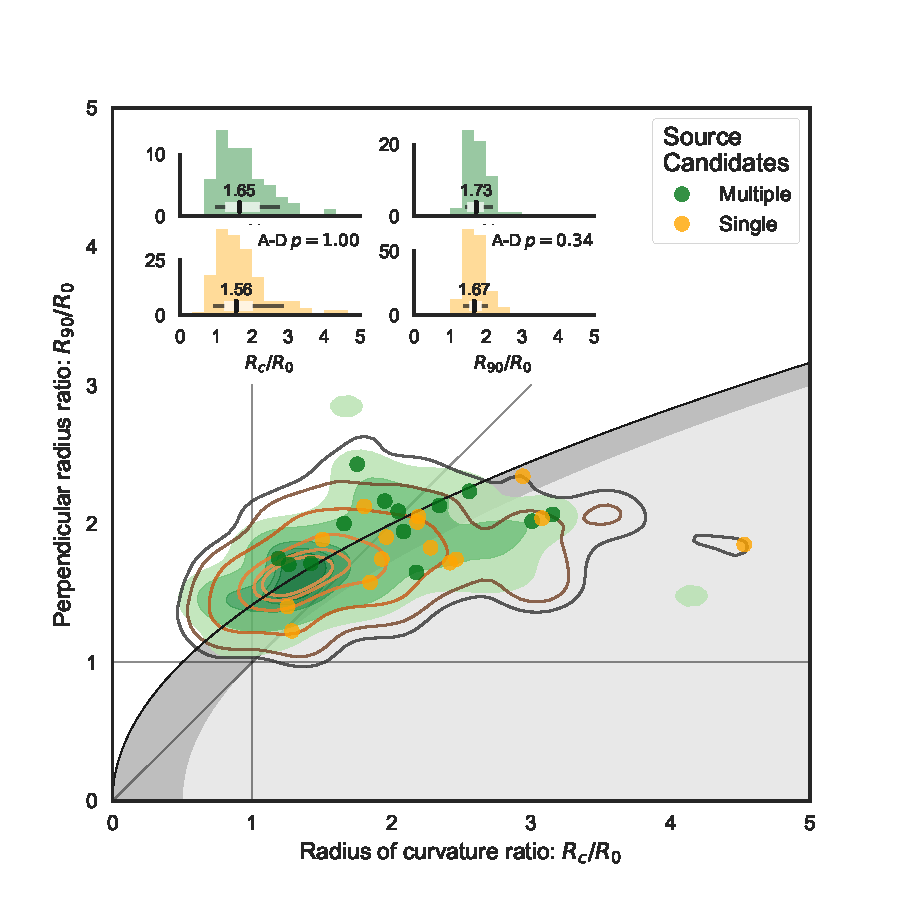
\includegraphics[width=0.45\textwidth]{figs/mipsgal-Rc-R90-candidates} 
  \end{tabular}
  \caption[]{Lack of significant correlation of bow shock shape with
    (a) environment, and (b) uncertainty in stellar source
    identification.}
  \label{fig:mipsgal-uncorrelated}
\end{figure*}


\subsection{Far-infrared arcs around late-type stars}
\label{sec:far-infrared-arcs}

\subsection{Stationary emission line arcs in M42}
\label{sec:stat-emiss-line}

\begin{figure*}
  \centering
  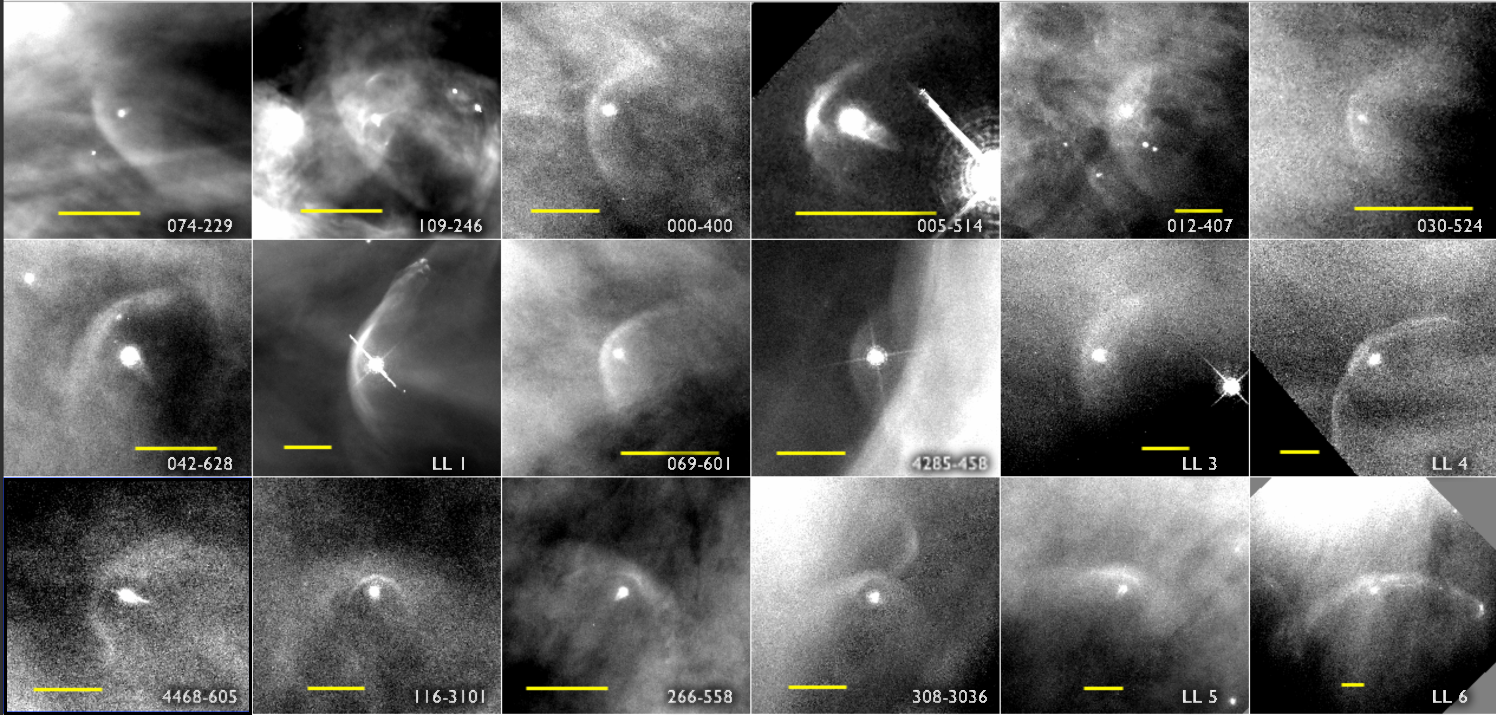
\includegraphics[width=\textwidth]{figs/annotated-ll-arcs}
  \caption[]{Stationary bow shock arcs in the Orion Nebula}
  \label{fig:ll-arcs}
\end{figure*}

\begin{figure}
  \centering
  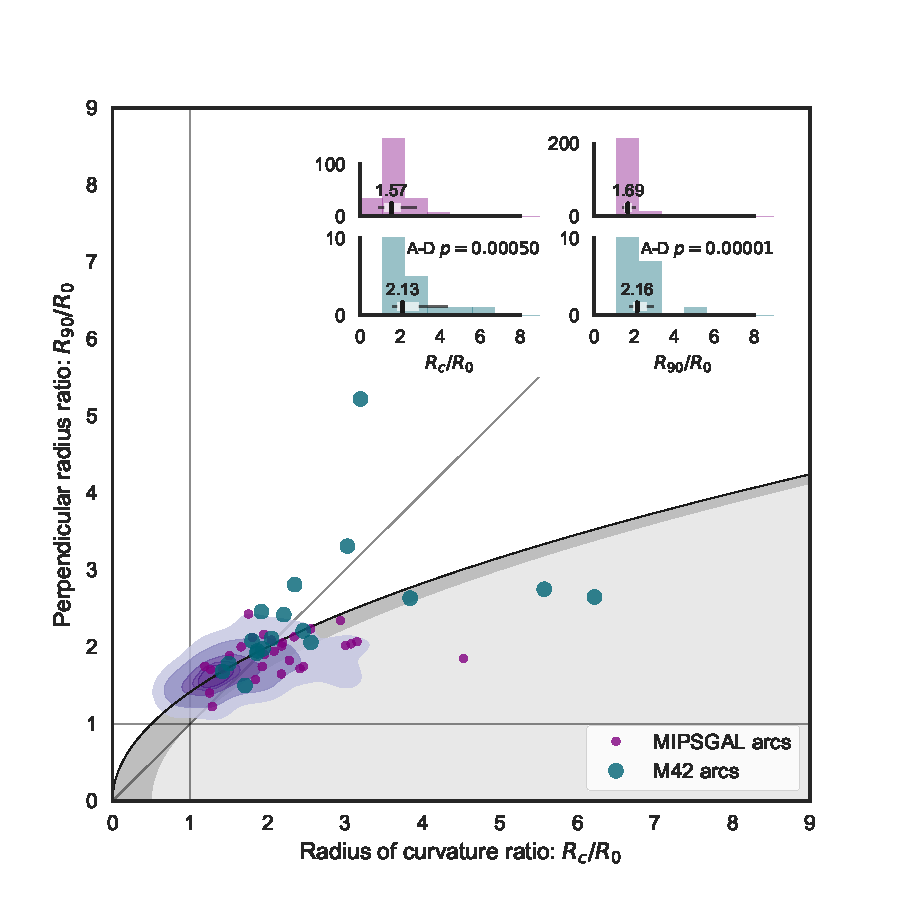
\includegraphics[width=\linewidth]{figs/mipsgal-Rc-R90-vs-Orion}
  \caption[]{Comparison of Orion with OB stars}
  \label{fig:ll-compare-mipsgal}
\end{figure}




%%% Local Variables:
%%% mode: latex
%%% TeX-master: "quadrics-bowshock.tex"
%%% End:
